% !TeX root = booklet-03.tex
\clearpage
\subsection{اثر نسبت \lr{Beta}}
\label{sec:beta-ratio}
در بخش قبل، \(\beta_n=\beta_p\) و بزرگی دو آستانه برابر بود.
اکنون نسبت قدرت دو مسیر را تغییر می‌دهیم و اثر آن بر
\(V_{\mathrm{inv}}\) را استخراج می‌کنیم. مبنای این بخش، روابط
\secnum{۲.۵۴} تا \secnum{۲.۵۷}، شکل \secnum{۲.۲۸} کتاب و
اسلاید ۸ است \cite[بخش \secnum{۲.۵.۲}، صفحات ۹۰ و ابتدای ۹۱]{weste}
\cite[اسلاید ۸]{dcslides}. همه جریان‌ها با قرارداد مثبت
\(I_n=I_{DS,n}\) و \(I_p=|I_{DS,p}|\) بخش
\ref{sec:inverter-conventions} نوشته می‌شوند.

\subsubsection{معنای نسبت و \lr{Skew}}
\label{sec:beta-skew-definition}
نسبت \lr{Beta} در مدل \lr{Long-channel} را چنین تعریف می‌کنیم
\begin{equation}
 \boxed{r_\beta=\frac{\beta_p}{\beta_n}}>0.
 \label{eq:beta-ratio-definition}
\end{equation}
هر دو \(\beta\) واحد \(\unit{\ampere\per\volt\squared}\) دارند،
پس \(r_\beta\) بی‌بعد است. مثلاً اگر
\(\beta_n=\qty{200}{\micro\ampere\per\volt\squared}\) و
\(\beta_p=\qty{800}{\micro\ampere\per\volt\squared}\) باشند،
\(r_\beta=4\) است. در اضافه‌ولتاژ گیت و ناحیه کاری یکسان،
ضریب جریان \lr{pMOS} در این مدل چهار برابر است.

در قرارداد کتاب، \(r_\beta>1\) را \lr{HI-skewed}،
\(r_\beta<1\) را \lr{LO-skewed} و \(r_\beta=1\) را
\lr{Unskewed} می‌نامند \cite[صفحه ۹۰]{weste}.
برای آستانه‌های با بزرگی برابر، \lr{HI-skewed} مسیر بالاکش
قوی‌تری دارد. در ورودی میانی، افزایش جریان بالاکش، بار خروجی
را بیشتر می‌کند و خروجی بالاتر می‌رود. برای برقراری دوباره تعادل
در شرط \(V_{\mathrm{out}}=V_{\mathrm{in}}\)، باید ورودی بالاتر
رود تا جریان \lr{nMOS} بیشتر و جریان \lr{pMOS} کمتر شود.
پس آستانه ورودی به سمت ولتاژ بالاتر جابه‌جا می‌شود.
در \lr{LO-skewed}، جهت جابه‌جایی معکوس است.

برابری \(\beta\) و بزرگی آستانه‌ها، تقارن دو مسیر را در مدل
ساده ایجاد می‌کند. مرجع این تقارن را برای حاشیه‌های منطقی
متوازن و توانایی مشابه شارژ و تخلیه بار خازنی مطلوب می‌داند
\cite[آغاز بخش \secnum{۲.۵.۲}]{weste}.
برابری زمان شارژ و تخلیه به تقارن مدل جریان، بار و شرایط تحریک
نیز وابسته است. تحلیل حاشیه‌های منطقی در بخش \secnum{۲.۵.۳}
تکمیل می‌شود.

\subsubsection{استخراج آستانه در مدل \lr{Long-channel}}
\label{sec:beta-long-channel}
برای جلوگیری از اشتباه علامت، دو ولتاژ مرزی را تعریف می‌کنیم
\begin{equation}
 L=V_{tn},\qquad H=V_{DD}-V_{TP}=V_{DD}+V_{tp},\qquad
 \Delta=H-L>0.
 \label{eq:beta-window}
\end{equation}
نمادهای \(L\) و \(H\) در این بخش ولتاژند. طول کانال در روابط
هندسی با زیرنویس افزاره، مانند \(L_n\)، نوشته می‌شود.
بازه \(L<V_{\mathrm{in}}<H\) بازه روشن‌بودن هم‌زمان دو
افزاره در مدل هدایت قوی است. شرط \(\Delta>0\) یعنی
\(V_{DD}>V_{tn}+V_{TP}\).

آستانه ورودی با \(V_{\mathrm{in}}=V_{\mathrm{out}}=M\) تعریف
می‌شود که در این بخش \(M=V_{\mathrm{inv}}\) است.
در این نقطه، \lr{nMOS} روشن شرط اشباع را خودبه‌خود دارد، زیرا
\(V_{DS,n}=M\ge M-V_{tn}\). برای \lr{pMOS} نیز
\(V_{SD,p}=V_{DD}-M\ge V_{DD}-M-V_{TP}\) برقرار است.
پس اگر \(L<M<H\) باشد، هر دو در اشباع‌اند.
با استفاده از مدل مربعی رابطه \secnum{۲.۵۴} کتاب می‌نویسیم
\begin{equation}
 I_n=\frac{\beta_n}{2}(M-L)^2,\qquad
 I_p=\frac{\beta_p}{2}(H-M)^2.
 \label{eq:beta-long-currents}
\end{equation}
در قرارداد علامت‌دار کتاب، جریان \lr{pMOS} در جهت درین به
سورس منفی است. برابری بزرگی جریان‌ها در قرارداد حاضر، همان
\lr{KCL} گره خروجی را اعمال می‌کند.

تقسیم دو طرف معادله جریان بر \(\beta_n/2>0\) می‌دهد
\begin{align}
 (M-L)^2&=r_\beta(H-M)^2,\notag\\
 M-L&=\sqrt{r_\beta}(H-M).
 \label{eq:beta-positive-root}
\end{align}
در سطر دوم از مثبت‌بودن هر دو اضافه‌ولتاژ استفاده شده است.
اگر صرفاً از برابری مربع‌ها ریشه مثبت و منفی بگیریم، باید شرط
روشن‌بودن هر دو افزاره را هم اعمال کنیم. در بازه مورد نظر،
\(M-L>0\) و \(H-M>0\) هستند و علامت مثبت لازم است.

با تعریف \(s=\sqrt{r_\beta}>0\)، جمله‌های شامل \(M\) را جمع می‌کنیم
\begin{align}
 M-L&=sH-sM,\notag\\
 M+sM&=L+sH,\notag\\
 \boxed{M=\frac{L+sH}{1+s}
 =\frac{V_{tn}+\sqrt{r_\beta}(V_{DD}-V_{TP})}
              {1+\sqrt{r_\beta}}}.
 \label{eq:beta-long-threshold}
\end{align}
صورت واحد ولت و مخرج بی‌بعد دارد. با تقسیم صورت و مخرج بر
\(s\) و جای‌گذاری \(V_{TP}=-V_{tp}\)، شکل نوشته‌شده در
رابطه \secnum{۲.۵۵} کتاب به دست می‌آید
\begin{equation}
 M=\frac{V_{DD}+V_{tp}+V_{tn}\sqrt{1/r_\beta}}
              {1+\sqrt{1/r_\beta}}.
 \label{eq:beta-book-long-form}
\end{equation}
عبارت \(V_{DD}+V_{tp}\)، با منفی‌بودن \(V_{tp}\)، همان
\(V_{DD}-V_{TP}\) است.

\paragraph*{کنترل جواب و رفتار حدی}
برای اثبات قرارگرفتن جواب در دامنه، از
\eqref{eq:beta-long-threshold} دو تفاضل را محاسبه می‌کنیم
\begin{equation}
 M-L=\frac{s\Delta}{1+s}>0,\qquad
 H-M=\frac{\Delta}{1+s}>0.
 \label{eq:beta-threshold-domain}
\end{equation}
پس فرض روشن‌بودن و اشباع هم‌زمان سازگار است. همچنین \(M\)
یک میانگین وزنی از دو ولتاژ مرزی است. افزایش وزن \(H\)، جواب
را به سمت \(H\) می‌برد. برای \(r_\beta\to0^+\)،
\(M\to L\) و برای \(r_\beta\to\infty\)، \(M\to H\).
این دو، حد نسبت‌های مثبت‌اند. اگر یکی از ضریب‌های جریان دقیقاً
صفر باشد، فرض وجود دو مسیر فعال باید دوباره بررسی شود.

در \(r_\beta=1\)، جواب برابر است با
\begin{equation}
 M=\frac{L+H}{2}
   =\frac{V_{DD}+V_{tn}-V_{TP}}{2}.
 \label{eq:beta-equal-strength}
\end{equation}
برای \(V_{tn}=V_{TP}\)، مقدار \(V_{DD}/2\) بازیابی می‌شود.
بنابراین، ادعای آستانه میانی با \(r_\beta=1\)، فرض برابری
بزرگی آستانه‌ها را نیز در خود دارد.

\paragraph*{مثال آموزشی آستانه و کنترل دو جریان}
فرض کنید \(V_{DD}=\qty{1.2}{\volt}\)،
\(V_{tn}=V_{TP}=\qty{0.3}{\volt}\)،
\(\beta_n=\qty{200}{\micro\ampere\per\volt\squared}\) و
\(\beta_p=\qty{800}{\micro\ampere\per\volt\squared}\) باشند.
این پارامترها برای آموزش فرض شده‌اند. داریم
\(L=\qty{0.3}{\volt}\)، \(H=\qty{0.9}{\volt}\)،
\(r_\beta=4\) و \(s=2\). پس
\begin{equation*}
 M=\frac{0.3+2(0.9)}{1+2}=\qty{0.7}{\volt}.
\end{equation*}
اضافه‌ولتاژ \lr{nMOS} برابر \(\qty{0.4}{\volt}\) و
اضافه‌ولتاژ \lr{pMOS} برابر \(\qty{0.2}{\volt}\) است.
در \(V_{\mathrm{out}}=M\)، ولتاژهای درین و سورس متناظر
\(V_{DS,n}=\qty{0.7}{\volt}\) و
\(V_{SD,p}=\qty{0.5}{\volt}\) هستند، پس هر دو شرط اشباع برقرارند.
کنترل مستقل جریان‌ها می‌دهد
\begin{equation*}
 I_n=(200/2)(0.4)^2=\qty{16}{\micro\ampere},\qquad
 I_p=(800/2)(0.2)^2=\qty{16}{\micro\ampere}.
\end{equation*}
قوی‌ترشدن مسیر \lr{pMOS}، آستانه را از
\(\qty{0.6}{\volt}\) در حالت متقارن به
\(\qty{0.7}{\volt}\) رسانده است.

\subsubsection{اثر نسبت بر تمام مشخصه انتقال}
\label{sec:beta-transfer-curves}
در مدل ایده‌آل، تغییر نسبت، محل گذار تند را جابه‌جا می‌کند.
برای نشان‌دادن این اثر، استخراج ناحیه‌های \lr{B} و \lr{D}
بخش \ref{sec:inverter-five-regions} را با دو ضریب متفاوت انجام
می‌دهیم. همچنان \(a=V_{\mathrm{in}}-V_{tn}\)،
\(b=V_{DD}-V_{\mathrm{in}}-V_{TP}\)،
\(u=V_{DD}-y\) و \(y=V_{\mathrm{out}}\) هستند.
در \lr{B}، \lr{nMOS} در اشباع و \lr{pMOS} در \lr{Linear} است.
پس
\begin{align}
 \frac{\beta_n a^2}{2}&=\beta_p(bu-u^2/2),\notag\\
 u^2-2bu+\frac{a^2}{r_\beta}&=0,\notag\\
 \boxed{y=V_{DD}-b+\sqrt{b^2-a^2/r_\beta}}.
 \label{eq:beta-b-transfer}
\end{align}
ریشه انتخاب‌شده همان ریشه‌ای است که \(0\le u\le b\) می‌دهد.
در \(L<V_{\mathrm{in}}<M\)، رابطه
\(a<\sqrt{r_\beta}b\) برقرار است و رادیکال حقیقی می‌ماند.
در \lr{D}، با \lr{nMOS} در \lr{Linear} و \lr{pMOS} در
اشباع، داریم
\begin{align}
 \beta_n(ay-y^2/2)&=\frac{\beta_pb^2}{2},\notag\\
 y^2-2ay+r_\beta b^2&=0,\notag\\
 \boxed{y=a-\sqrt{a^2-r_\beta b^2}}.
 \label{eq:beta-d-transfer}
\end{align}
در \(M<V_{\mathrm{in}}<H\)، رادیکال حقیقی و ریشه مجاز در
\(0\le y\le a\) است. در نقطه گذار \(V_{\mathrm{in}}=M\)،
خروجی‌های اشباع هم‌زمان در بازه زیر قرار دارند
\begin{equation}
 M-V_{tn}\le y\le M+V_{TP}.
 \label{eq:beta-c-interval}
\end{equation}
در ورودی‌های \(V_{\mathrm{in}}\le L\)، خروجی ایده‌آل
\(V_{DD}\) و در \(V_{\mathrm{in}}\ge H\)، خروجی صفر است.
شرط‌های هر شاخه با روش بخش قبل کنترل می‌شوند.

شکل \ref{fig:beta-vtc-family} سه مشخصه فرضی با
\(V_{tn}=V_{TP}=0.25V_{DD}\) را نشان می‌دهد. منحنی‌ها مستقیماً
از \eqref{eq:beta-b-transfer}، \eqref{eq:beta-d-transfer} و
\eqref{eq:beta-c-interval} رسم شده‌اند. این شکل، توضیح محاسباتی
روند شکل \secnum{۲.۲۸} کتاب و اسلاید ۸ است \cite{weste,dcslides}.
\begin{figure}[!htbp]
\centering
\begin{latin}
\PersianMathDigits
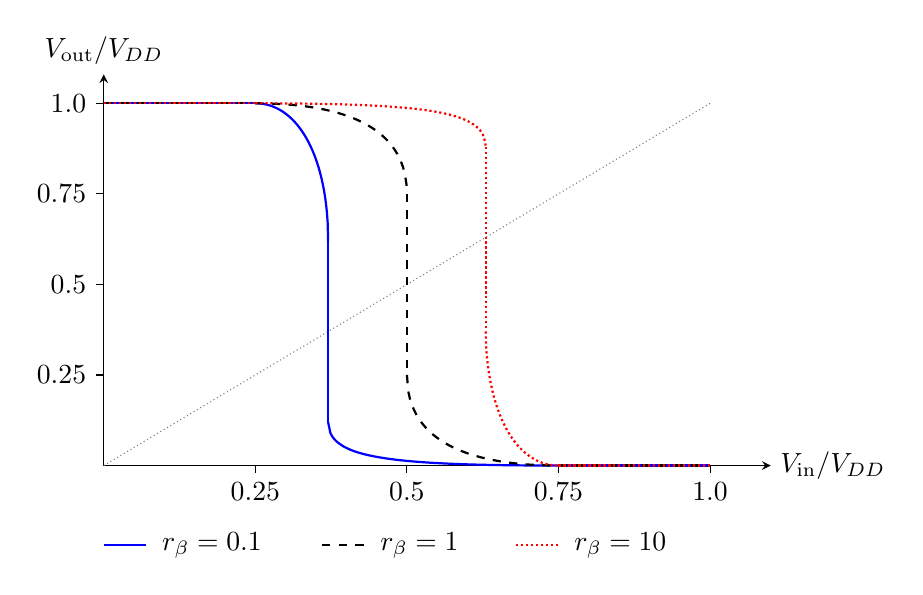
\begin{tikzpicture}[x=7.7cm,y=4.6cm,>=stealth,
 lowratio/.style={blue,thick},
 balancedratio/.style={black,thick,dashed},
 highratio/.style={red,thick,densely dotted}]
\draw[->] (0,0)--(1.10,0) node[right] {\(V_{\mathrm{in}}/V_{DD}\)};
\draw[->] (0,0)--(0,1.08) node[above] {\(V_{\mathrm{out}}/V_{DD}\)};
\foreach \x in {0.25,0.5,0.75,1.0}
 {\draw (\x,0)--(\x,-0.02) node[below] {\(\x\)};}
\foreach \y in {0.25,0.5,0.75,1.0}
 {\draw (0,\y)--(-0.013,\y) node[left] {\(\y\)};}
\draw[densely dotted,gray] (0,0)--(1,1);
\foreach \r/\curvestyle in {0.1/lowratio,1/balancedratio,10/highratio} {
 \pgfmathsetmacro{\m}{(0.25+sqrt(\r)*0.75)/(1+sqrt(\r))}
 \draw[\curvestyle] (0,1)--(0.25,1);
 \draw[\curvestyle,domain=0.25:\m,samples=100]
  plot (\x,{\x+0.25+sqrt(max(0,(0.75-\x)^2-(\x-0.25)^2/\r))})
  -- (\m,{\m+0.25});
 \draw[\curvestyle] (\m,{\m+0.25})--(\m,{\m-0.25});
 \draw[\curvestyle,domain=\m:0.75,samples=100]
  plot (\x,{\x-0.25-sqrt(max(0,(\x-0.25)^2-\r*(0.75-\x)^2))});
 \draw[\curvestyle] (0.75,0)--(1,0);
}
\draw[blue,thick] (0,-0.22)--(0.07,-0.22);
\node[anchor=west] at (0.08,-0.22) {\(r_\beta=0.1\)};
\draw[black,thick,dashed] (0.36,-0.22)--(0.43,-0.22);
\node[anchor=west] at (0.44,-0.22) {\(r_\beta=1\)};
\draw[red,thick,densely dotted] (0.68,-0.22)--(0.75,-0.22);
\node[anchor=west] at (0.76,-0.22) {\(r_\beta=10\)};
\end{tikzpicture}
\end{latin}
\caption{جابه‌جایی مشخصه انتقال با تغییر نسبت \lr{Beta} در مدل
مربعی ایده‌آل. محورها بی‌بعدند و خط مورب شرط
\(V_{\mathrm{out}}=V_{\mathrm{in}}\) را مشخص می‌کند.}
\label{fig:beta-vtc-family}
\end{figure}

\subsubsection{استخراج آستانه در حد \lr{Velocity Saturation}}
\label{sec:beta-velocity-limit}
در حد اشباع کامل سرعت، رابطه \secnum{۲.۲۹} کتاب جریان اشباع
را تقریباً متناسب با توان اول اضافه‌ولتاژ می‌دهد. با تعریف
\(K_n=W_nC_{\mathrm{ox},n}v_{\mathrm{sat},n}\) و
\(K_p=W_pC_{\mathrm{ox},p}v_{\mathrm{sat},p}\)، بزرگی دو جریان
رابطه \secnum{۲.۵۶} کتاب چنین نوشته می‌شود
\begin{equation}
 I_n=K_n(M-L),\qquad I_p=K_p(H-M).
 \label{eq:beta-velocity-currents}
\end{equation}
واحد \(K\) از حاصل‌ضرب
\(\mathrm{m}\times\mathrm{F\,m^{-2}}\times\mathrm{m\,s^{-1}}\)
برابر \(\mathrm{F\,s^{-1}}=\mathrm{A\,V^{-1}}\) است.
پس ضرب آن در ولتاژ، جریان می‌دهد.
این حد وقتی قابل استفاده است که محدودیت سرعت غالب باشد.
در \NotesTopic{sec:high-field}{مدل میدان قوی}، شرط متناظر
\(V_c\ll V_{GT}\) است و باید برای هر افزاره بررسی شود.

نسبت قدرت در این مدل را با نماد متمایز تعریف می‌کنیم
\begin{equation}
 \boxed{r_v=\frac{K_p}{K_n}
 =\frac{W_pC_{\mathrm{ox},p}v_{\mathrm{sat},p}}
        {W_nC_{\mathrm{ox},n}v_{\mathrm{sat},n}}}>0.
 \label{eq:beta-velocity-ratio}
\end{equation}
در فرض عایق گیت یکسان، \(C_{\mathrm{ox}}\) حذف می‌شود و همان
تعریف \(r=W_pv_{\mathrm{sat},p}/(W_nv_{\mathrm{sat},n})\)
صفحه ۹۰ کتاب به دست می‌آید. کتاب نماد \(r\) را در این مرحله
دوباره تعریف می‌کند. این جزوه از \(r_\beta\) و \(r_v\) استفاده
می‌کند تا مدل هر نسبت روشن باشد.

با برابرکردن جریان‌ها و تقسیم بر \(K_n>0\)، مراحل حل عبارت‌اند از
\begin{align}
 M-L&=r_v(H-M),\notag\\
 M+r_vM&=L+r_vH,\notag\\
 \boxed{M=\frac{L+r_vH}{1+r_v}
 =\frac{V_{tn}+r_v(V_{DD}-V_{TP})}{1+r_v}}.
 \label{eq:beta-velocity-threshold}
\end{align}
با تقسیم صورت و مخرج بر \(r_v\)، شکل رابطه \secnum{۲.۵۷}
کتاب حاصل می‌شود
\begin{equation}
 M=\frac{V_{DD}+V_{tp}+V_{tn}/r_v}{1+1/r_v}.
 \label{eq:beta-book-velocity-form}
\end{equation}
شرط دامنه نیز با
\(M-L=r_v\Delta/(1+r_v)>0\) و
\(H-M=\Delta/(1+r_v)>0\) تأیید می‌شود.
در \(r_v=1\) و آستانه‌های برابر، دوباره
\(M=V_{DD}/2\) است.

\paragraph*{مثال آموزشی مدل خطی اضافه‌ولتاژ}
فرض کنید حد اشباع کامل سرعت برای هر دو افزاره برقرار باشد،
\(V_{DD}=\qty{1.2}{\volt}\)،
\(V_{tn}=V_{TP}=\qty{0.3}{\volt}\)،
\(K_n=\qty{50}{\micro\ampere\per\volt}\) و
\(K_p=\qty{200}{\micro\ampere\per\volt}\).
این پارامترها یک مدل آموزشی مستقل را تعریف می‌کنند.
در \(r_v=4\)، داریم
\begin{equation*}
 M=\frac{0.3+4(0.9)}{5}=\qty{0.78}{\volt}.
\end{equation*}
اضافه‌ولتاژها \(\qty{0.48}{\volt}\) و \(\qty{0.12}{\volt}\) هستند.
برابری جریان‌ها با جای‌گذاری این دو مقدار کنترل می‌شود.
\[
 50(0.48)=200(0.12)=\qty{24}{\micro\ampere}.
\]
ولتاژهای \(V_{DS,n}=\qty{0.78}{\volt}\) و
\(V_{SD,p}=\qty{0.42}{\volt}\) از اضافه‌ولتاژهای متناظر بیشترند.
فرض محدودیت غالب سرعت، بخشی از مدل این مثال است.
تأیید آن در یک فناوری به پارامترهای \(V_c\) همان فناوری نیاز دارد.

\subsubsection{مقایسه حساسیت دو مدل و طراحی ابعاد}
\label{sec:beta-sensitivity-sizing}
جدول \ref{tab:beta-threshold-comparison} آستانه را با
\(L=\qty{0.3}{\volt}\) و \(H=\qty{0.9}{\volt}\) مقایسه می‌کند.
عدد نسبت در هر ستون، با تعریف همان مدل به کار رفته است.
قرارگرفتن دو مقدار برابر در یک ردیف، انتخاب آموزشی وزن‌های
بی‌بعد است. برای یک هندسه مشخص، باید هر نسبت جداگانه از
پارامترهای همان مدل محاسبه شود.
\begin{table}[!htbp]
\centering
\small
\caption{آستانه محاسبه‌شده از دو مدل برای نسبت‌های فرضی.
هر دو ستون آستانه برحسب \(\unit{\volt}\) هستند.}
\label{tab:beta-threshold-comparison}
\begin{tabular}{ccc}
\toprule
مقدار نسبت در مدل مربوط & \(M(r_\beta)\)، مدل مربعی & \(M(r_v)\)، حد سرعت\\
\midrule
\num{0.1} & \num{0.4442} & \num{0.3545}\\
\num{0.5} & \num{0.5485} & \num{0.5000}\\
\num{1} & \num{0.6000} & \num{0.6000}\\
\num{2} & \num{0.6515} & \num{0.7000}\\
\num{4} & \num{0.7000} & \num{0.7800}\\
\num{10} & \num{0.7558} & \num{0.8455}\\
\bottomrule
\end{tabular}
\end{table}

\paragraph*{استخراج حساسیت نزدیک نسبت یک}
مشتق \(\mathrm{d}M/\mathrm{d}r\)، تغییر آستانه در برابر تغییر
کوچک نسبت را اندازه می‌گیرد. برای مدل مربعی،
\(M=L+\Delta s/(1+s)\) و \(s=\sqrt{r_\beta}\) است.
مشتق \(s/(1+s)\) نسبت به \(s\) و مشتق ریشه به‌ترتیب چنین‌اند.
\[
 \frac{(1+s)-s}{(1+s)^2}=\frac{1}{(1+s)^2},\qquad
 \frac{\mathrm{d}s}{\mathrm{d}r_\beta}=\frac{1}{2\sqrt{r_\beta}}.
\]
با ضرب این دو نرخ، نتیجه می‌شود
\begin{equation}
 \frac{\mathrm{d}M}{\mathrm{d}r_\beta}
 =\frac{\Delta}{2\sqrt{r_\beta}(1+\sqrt{r_\beta})^2},\qquad
 \left.\frac{\mathrm{d}M}{\mathrm{d}r_\beta}\right|_{r_\beta=1}
 =\frac{\Delta}{8}.
 \label{eq:beta-long-sensitivity}
\end{equation}
برای مدل حد سرعت، \(M=L+\Delta r_v/(1+r_v)\) است، پس
\begin{equation}
 \frac{\mathrm{d}M}{\mathrm{d}r_v}
 =\frac{\Delta}{(1+r_v)^2},\qquad
 \left.\frac{\mathrm{d}M}{\mathrm{d}r_v}\right|_{r_v=1}
 =\frac{\Delta}{4}.
 \label{eq:beta-velocity-sensitivity}
\end{equation}
هر دو مشتق مثبت و دارای واحد ولت‌اند، زیرا نسبت بی‌بعد است.
در مقایسه حول نسبت یک و برای \(\Delta\) یکسان، حساسیت حد سرعت
دو برابر حساسیت مدل مربعی است. با \(\Delta=\qty{0.6}{\volt}\)،
شیب‌ها \(\qty{0.075}{\volt}\) و \(\qty{0.15}{\volt}\) به ازای
یک واحد تغییر نسبت‌اند. برای افزایش نسبت از یک به \num{1.1}،
تقریب خطی به‌ترتیب جابه‌جایی \(\qty{7.5}{\milli\volt}\) و
\(\qty{15}{\milli\volt}\) می‌دهد. محاسبه دقیق،
\(\qty{7.147}{\milli\volt}\) و
\(\qty{14.286}{\milli\volt}\) است.

مرجع حساسیت بیشتر مدارهای با محدودیت سرعت به \lr{Skew} را بیان
می‌کند \cite[پایان صفحه ۹۰]{weste}. مشتق‌های حاضر، این موضوع
را برای آستانه و نسبت‌های تعریف‌شده کمی می‌کنند.
شیب منحنی انتقال نسبت به ورودی، کمیت دیگری است و از
\eqref{eq:inverter-gain} و رسانایی‌های خروجی اثر می‌گیرد.
هر دو مدل ایده‌آل اشباع در استخراج آستانه، مستقل از خروجی‌اند و
در ناحیه اشباع هم‌زمان، گذار عمودی دارند. برای توصیف شیب محدود
مدار واقعی باید اثرهایی مانند \lr{CLM} نیز وارد شوند.

\paragraph*{از نسبت قدرت تا نسبت عرض}
رابطه هندسی مدل مربعی به صورت زیر است
\begin{equation}
 r_\beta=\frac{\mu_pC_{\mathrm{ox},p}}{\mu_nC_{\mathrm{ox},n}}
          \frac{W_p/L_p}{W_n/L_n}.
 \label{eq:beta-geometry-ratio}
\end{equation}
در طول و عایق یکسان،
\(r_\beta=(\mu_p/\mu_n)(W_p/W_n)\).
برای مثال فرضی \(\mu_p=0.5\mu_n\)، نسبت عرض دو،
\(r_\beta=1\) و نسبت عرض هشت، \(r_\beta=4\) می‌دهد.
کتاب معمولاً تغییر عرض با نگه‌داشتن طول کمینه مناسب فناوری را
برای تنظیم \lr{Skew} مطرح می‌کند \cite[صفحه ۹۰]{weste}.
تغییر طول هم‌زمان بر جریان، ظرفیت و اثرهای کانال کوتاه اثر دارد.
مقادیر ابعاد باید با تعریف ابعاد مؤثر مدل سازگار باشند.

در حد سرعت و با عایق یکسان،
\(r_v=(v_{\mathrm{sat},p}/v_{\mathrm{sat},n})(W_p/W_n)\).
اگر به‌طور آموزشی \(v_{\mathrm{sat},p}=0.8v_{\mathrm{sat},n}\)
و \(W_p/W_n=2\) فرض شوند، \(r_v=1.6\) است.
با \(\mu_p/\mu_n=0.5\)، همین نسبت عرض در مدل مربعی
\(r_\beta=1\) داشت. برای آستانه‌های \(\qty{0.3}{\volt}\) و
تغذیه \(\qty{1.2}{\volt}\)، نتیجه رسمی مدل مربعی
\(M=\qty{0.6}{\volt}\) است. محاسبه در حد سرعت می‌دهد
\[
 M=\frac{0.3+1.6\times0.9}{2.6}\approx\qty{0.6692}{\volt}.
\]
برای کاربرد هر حد باید دامنه اعتبار آن بررسی شود.

\paragraph*{طراحی معکوس برای آستانه مطلوب}
اگر آستانه هدف \(M_\star\) در \(L<M_\star<H\) باشد، از
\eqref{eq:beta-positive-root} و مدل حد سرعت به دست می‌آید
\begin{equation}
 \boxed{r_\beta=\left(\frac{M_\star-L}{H-M_\star}\right)^2},\qquad
 \boxed{r_v=\frac{M_\star-L}{H-M_\star}}.
 \label{eq:beta-inverse-sizing}
\end{equation}
هر دو کسر بی‌بعد و مثبت‌اند. نزدیک‌شدن هدف به \(H\)، مخرج را
کوچک و نسبت مورد نیاز را بزرگ می‌کند.
برای \(M_\star=\qty{0.65}{\volt}\)، \(L=\qty{0.3}{\volt}\)
و \(H=\qty{0.9}{\volt}\)، نسبت اضافه‌ولتاژها چنین محاسبه می‌شود.
\[
 \frac{0.65-0.3}{0.9-0.65}=\frac{0.35}{0.25}=1.4.
\]
پس \(r_\beta=1.96\) و \(r_v=1.4\) لازم است.
در مدل مربعی با \(\mu_p/\mu_n=0.5\)، طول و عایق یکسان،
نسبت عرض‌ها به دست می‌آید.
\[
 \frac{W_p}{W_n}=\frac{1.96}{0.5}=3.92.
\]
اگر \(W_n=\qty{0.4}{\micro\metre}\)،
\(W_p=\qty{1.568}{\micro\metre}\) خواهد بود.
این ابعاد، نتیجه مدل آموزشی‌اند و گردکردن ابعاد واقعی تابع قواعد
فناوری است. افزایش عرض، ظرفیت و مساحت را هم تغییر می‌دهد.

\subsubsection{تبدیل گیت‌های دیگر به \lr{Equivalent Inverter}}
\label{sec:beta-equivalent-inverter}
انتهای بخش \secnum{۲.۵.۲} کتاب و اسلاید ۸، تحلیل گیت‌های دیگر
با یک \lr{Equivalent Inverter} را مطرح می‌کنند
\cite[صفحه ۹۰ و آغاز ۹۱]{weste}\cite[اسلاید ۸]{dcslides}.
ابتدا ورودی‌های ثابت و متغیر و مسیرهای روشن را مشخص می‌کنیم.
چند ترانزیستور موازی روشن با بایاس‌های یکسان، جریان‌هایشان را جمع
می‌کنند و در مدل ساده، عرض مؤثر بیشتری می‌دهند. اگر تنها یک
شاخه موازی روشن باشد، شاخه‌های خاموش در جریان هدایت ایده‌آل
سهم صفر دارند. ظرفیت و نشتی آن شاخه‌ها در تحلیل‌های مربوط به
خود همچنان مطرح‌اند.

برای افزاره‌های یکسان موازی با گیت مشترک،
\(\beta_{\mathrm{eq}}=m\beta\) است که \(m\) تعداد واحدهای روشن
است. برای \(m\) واحد یکسان سری با گیت مشترک، در مدل
\lr{Shockley} با آستانه ثابت و بدون اثر بدنه و \lr{CLM}،
معادل طول \(mL_n\) یا \(mL_p\) و ضریب
\(\beta_{\mathrm{eq}}=\beta/m\) به کار می‌رود.
این نتیجه با برابری جریان‌ها و جمع افت ولتاژهای کانال سازگار است.
در مدل‌های غیرایده‌آل، به‌ویژه با اثر بدنه و محدودیت سرعت،
باید ناحیه کاری و گره‌های داخلی دوباره بررسی شوند.

\paragraph*{پیش‌نیاز \lr{NAND} و \lr{NOR}}
گیت دوورودی \lr{NAND}، متمم \lr{AND} است. خروجی فقط وقتی
صفر می‌شود که هر دو ورودی یک باشند. گیت \lr{NOR}، متمم
\lr{OR} است و خروجی فقط وقتی یک می‌شود که هر دو ورودی صفر
باشند. در پیاده‌سازی \lr{Static CMOS}، \lr{NAND} دو
\lr{nMOS} سری در شبکه پایین‌کش و دو \lr{pMOS} موازی در
شبکه بالاکش دارد. \lr{NOR} دو \lr{nMOS} موازی و دو
\lr{pMOS} سری دارد \cite[فصل ۱، بخش \secnum{۱.۴}]{weste}.
در مثال آموزشی حاضر، دو ورودی هر گیت به یک ولتاژ مشترک
\(v\) وصل می‌شوند تا مشخصه \(y(v)\) تک‌ورودی تعریف شود.

فرض کنید همه \lr{nMOS}ها ضریب \(\beta_n\) و همه
\lr{pMOS}ها ضریب \(\beta_p\) داشته باشند. با مدل سری و
موازی بیان‌شده، جدول \ref{tab:beta-equivalent-gates} حاصل می‌شود.
\begin{table}[!htbp]
\centering
\small
\caption{معادل آموزشی گیت‌ها با هر دو ورودی متصل به \(v\).
اثر بدنه، نشتی و \lr{CLM} صفر و آستانه‌ها ثابت‌اند.}
\label{tab:beta-equivalent-gates}
\begin{tabular}{cccc}
\toprule
گیت & \(\beta_{n,\mathrm{eq}}\) & \(\beta_{p,\mathrm{eq}}\) & نسبت معادل\\
\midrule
\lr{Inverter} & \(\beta_n\) & \(\beta_p\) & \(r_\beta\)\\
\lr{NAND} دوورودی & \(\beta_n/2\) & \(2\beta_p\) & \(4r_\beta\)\\
\lr{NOR} دوورودی & \(2\beta_n\) & \(\beta_p/2\) & \(r_\beta/4\)\\
\bottomrule
\end{tabular}
\end{table}
برای نمونه فرضی با \(r_\beta=1\)،
\(V_{tn}=V_{TP}=\qty{0.3}{\volt}\) و
\(V_{DD}=\qty{1.2}{\volt}\)، نسبت \lr{NAND} برابر چهار و
آستانه آن \(\qty{0.7}{\volt}\) است.
نسبت \lr{NOR} برابر \num{0.25} است. آستانه آن از رابطه مدل محاسبه می‌شود.
\[
 \frac{0.3+0.5\times0.9}{1.5}=\qty{0.5}{\volt}.
\]
این مقایسه به اتصال هر دو ورودی به \(v\) و فرض‌های مدل وابسته
است. وقتی یک ورودی ثابت و دیگری متغیر باشد، ولتاژ گیت‌های
افزاره‌های سری یکسان نیست و معادل ساده باید با تحلیل مدار
همان حالت ارزیابی شود.

\subsubsection{تمرین‌های تشریحی و کنترل نهایی}
\label{sec:beta-practice}
\paragraph*{تمرین آموزشی ۱ و آستانه‌های نابرابر}
با \(V_{DD}=\qty{1.2}{\volt}\)،
\(V_{tn}=\qty{0.35}{\volt}\)،
\(V_{TP}=\qty{0.25}{\volt}\) و \(r_\beta=4\)، آستانه
ورودی را در مدل مربعی حساب کنید.

\textbf{پاسخ.}
\(L=\qty{0.35}{\volt}\)، \(H=\qty{0.95}{\volt}\) و
\(s=2\) هستند. بنابراین،
\[
 M=\frac{0.35+2\times0.95}{3}=\qty{0.75}{\volt}.
\]
اضافه‌ولتاژها \(\qty{0.4}{\volt}\) و
\(\qty{0.2}{\volt}\) می‌شوند و نسبت مربع آن‌ها چهار است.
در \(y=M\)، \(V_{DS,n}=\qty{0.75}{\volt}\) و
\(V_{SD,p}=\qty{0.45}{\volt}\) از اضافه‌ولتاژها بیشترند.
پس هر دو شرط اشباع برقرار و \lr{KCL} سازگار است.

\paragraph*{تمرین آموزشی ۲ و یک نسبت از دو کمیت متفاوت}
فرض کنید \(\beta_p/\beta_n=4\). آیا می‌توان همین عدد را در
رابطه \eqref{eq:beta-velocity-threshold} گذاشت؟

\textbf{پاسخ.}
رابطه مذکور به \(r_v=K_p/K_n\) نیاز دارد. مقدار آن از
عرض‌ها، \(C_{\mathrm{ox}}\) و سرعت‌های اشباع به دست می‌آید.
برای نمونه با عایق و طول یکسان،
\(\mu_p/\mu_n=0.5\) و \(W_p/W_n=8\)،
\(r_\beta=4\) می‌شود. اگر
\(v_{\mathrm{sat},p}/v_{\mathrm{sat},n}=0.8\) هم فرض شود،
\(r_v=6.4\) است. برای \(L=\qty{0.3}{\volt}\) و
\(H=\qty{0.9}{\volt}\)، محاسبه در حد سرعت می‌دهد
\[
 M=\frac{0.3+6.4\times0.9}{7.4}\approx\qty{0.8189}{\volt}.
\]
اعتبار حد سرعت باید برای افزاره‌های مسئله برقرار باشد.

\paragraph*{تمرین آموزشی ۳ و بررسی هدف طراحی}
برای \(L=\qty{0.3}{\volt}\) و \(H=\qty{0.9}{\volt}\)،
هدف \(M_\star=\qty{0.95}{\volt}\) را بررسی کنید.

\textbf{پاسخ.}
هدف از \(H\) بیشتر است. در آن ورودی، افزاره \lr{pMOS} در
مدل هدایت قوی خاموش است و فرض استخراج اشباع هم‌زمان برقرار
نیست. رابطه میانگین وزنی \eqref{eq:beta-long-threshold} برای
نسبت مثبت، جواب را در \(L<M<H\) قرار می‌دهد.
پس این هدف با تغییر نسبت مثبت در همین مدل قابل دستیابی نیست.
مربع‌کردن کسر منفی در فرمول معکوس، شرط دامنه را برطرف نمی‌کند.

بخش \secnum{۲.۵.۳}، ارتباط مشخصه انتقال با بازه‌های معتبر
منطقی و تحمل نویز را بررسی می‌کند.
